\documentclass[11pt]{article}
\usepackage[margin=1in]{geometry}
\usepackage{graphicx}
\begin{document}
\section*{R89 bidirectional rank-32 transport: rejected pole bound}
The frozen \texttt{transport89-01} attempt stopped at column 1 in both
directions with pole-bound-exhausted errors at bound 51. The native log has
two Singular errors. Its late pass marker is invalid: the driver rejected
the run. There are zero accepted column images out of 64 requested.

\begin{center}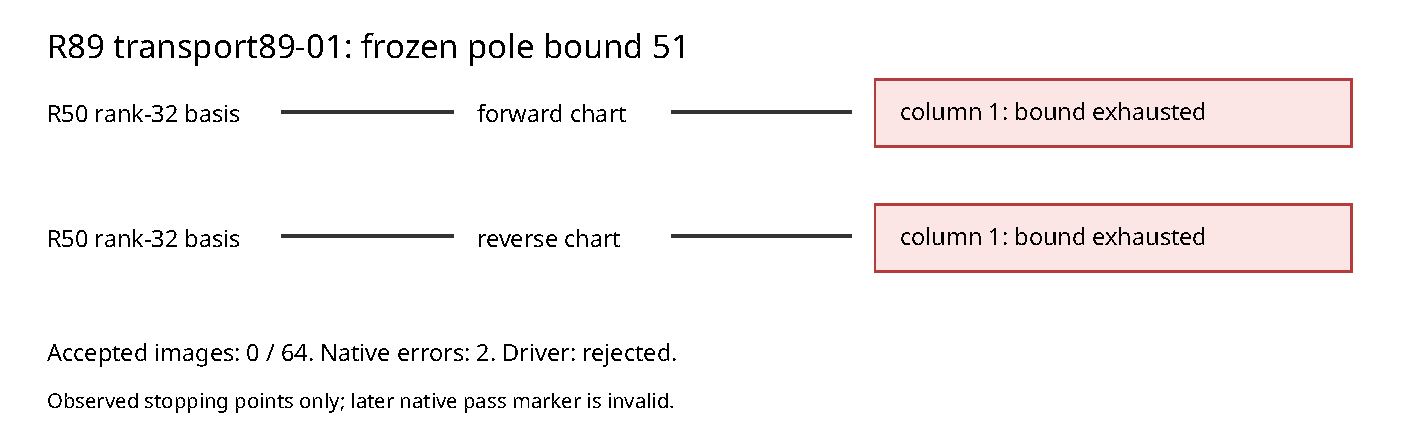
\includegraphics[width=\textwidth]{diagram.pdf}\end{center}

The source revision is \texttt{a624ea54235799a37e5c2488679d3e1ea7323b5e}.
The run used the R50 rank-32 PID basis and R85--R88 diamond maps, seed 89,
one thread, 4 GiB virtual memory and a 1200-second cap. The raw archive
contains the source and log; all 18 member hashes passed fresh readback.

The post-run bound calculation gives the conservative upper bound 61 from
the saved R27 cusp valuations and R50 relative degree. A new frozen attempt
must test that bound and stop fatally on the first native error. See
\texttt{BOUND-ERRATUM.md} and \texttt{CM.md} for evidence and derivation.
\end{document}
